\section{From MOONS to Sloan : Reminder} \label{reminder}

This section aims at explaining the differences between the MOONS project and the Sloan one, to understand the path taken in the rest of the project.
\\

MOONS (Multi-Object Optical and Near-infrared Spectrograph) is a design for the Very Large Telescope, the European Southern Observatory telescope facility. The fiber system is made of 1'000 actuators whose role is to position fibers on the surface of the telescope. Each actuator has two degrees of freedom as shown on Figure \ref{fig:reminder:actuator}. At the end of the second arm, each ferule contained only one near-IR fiber. The actuator structure had an hexagonal shape, with several holes for camera and fiducial tools.
\\

\begin{figure}[h]
\begin{center}
	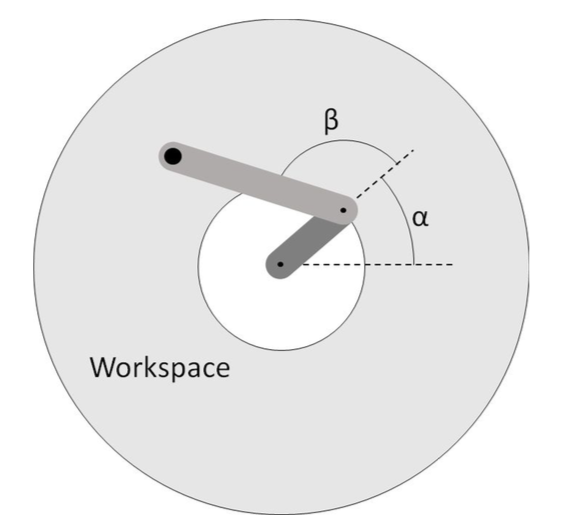
\includegraphics[width=0.40\textwidth]{reminder/actuator.png}
	\caption{Actuator's design, with the two degrees of freedom being $\alpha$ and $\beta$ angles. The arm displaced on the $\alpha$ angle is the $\alpha$-arm, while the arm displaced on the $\beta$ angle is the $\beta$-arm. The black dot at the end of the $\beta$-arm is the ferule, containing two to three fibers.}
	\label{fig:reminder:actuator}
\end{center}
\end{figure}

\begin{figure}[h]
\begin{center}
	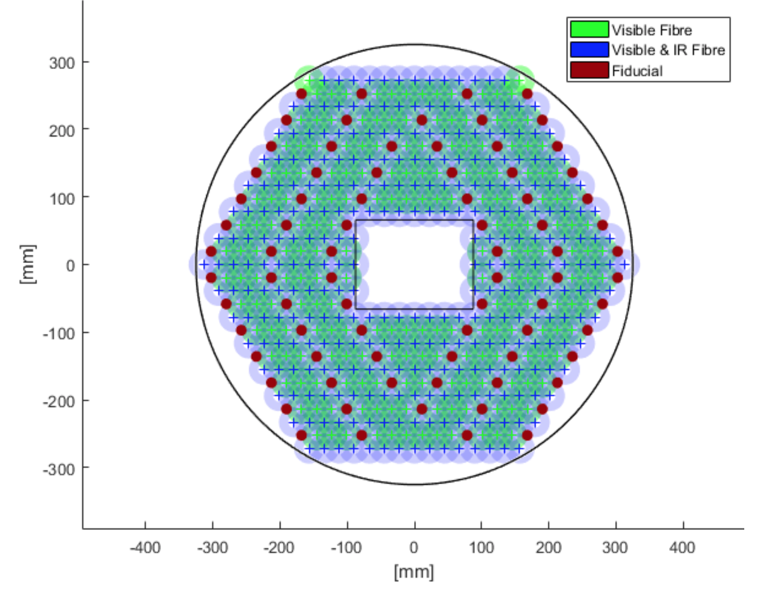
\includegraphics[width=\textwidth]{reminder/sloan_arrangement.png}
	\caption{Actuators structure for the Sloan project.}
	\label{fig:reminder:sloan_arrangement}
\end{center}
\end{figure}

\begin{figure}[h]
\begin{center}
	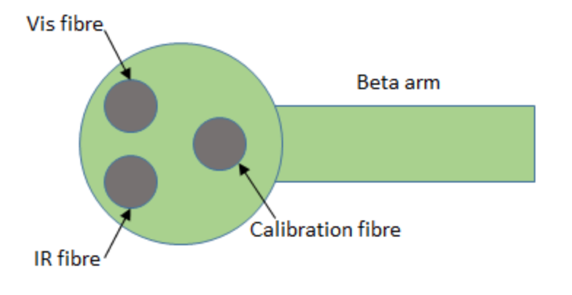
\includegraphics[width=0.40\textwidth]{reminder/ferule.png}
	\caption{Ferule design for the Sloan project.}
	\label{fig:reminder:ferule}
\end{center}
\end{figure}


For the Sloan telescope, the arrangement, as seen on Figure \ref{fig:reminder:sloan_arrangement}, is also hexagonal. However, the system is made of 500 actuators, with a rectangle in the middle of the telescope. Some actuator slots are taken by fiducial tools, in red on Figure \ref{fig:reminder:sloan_arrangement}.\\

The main update from the Sloan system is the presence of two to three fibers on each ferule. As shown on Figure \ref{fig:reminder:sloan_arrangement}, each ferule contains both a visible and a calibration fiber, while 300 of the 500 motors contain an additional IR fiber. This structure allows a spatial coverage by IR fibers of 99.5\% of the surface reachable by actuators, even if IR fibers are present only on three fifth of the actuators. A scheme of the new ferule is shown on Figure \ref{fig:reminder:ferule}.

